\documentclass[11pt]{article}
\parindent=0pt \parskip=8pt
%\textwidth=6.5in
%\hoffset=.3in
\usepackage{amssymb,amsmath,amsthm,mathrsfs}
\usepackage[margin=.75in]{geometry}
\usepackage{enumitem}
\setlist{topsep=0pt,parsep=0pt,partopsep=0pt,itemindent=0pt}
\usepackage{tikz}
\usetikzlibrary{arrows,calc}
\tikzset{>=stealth}

\pagestyle{plain}
\title{Is this object a circle?}
\author{}
\date{}

\begin{document}
\newgeometry{top= 0.75in, bottom=.75in, right=.75in, left=.75in}

%%%%%%%%%%%%%%%%%%%%%%%%%%%%%%%%%%%%%%%%%%%%%%%
%%%%%%%%%%%%%%%% NEW COMMANDS %%%%%%%%%%%%%%%%%

%Sets
\newcommand{\A}{\mathbb{A}}
\newcommand{\B}{\mathbb{B}}
\newcommand{\C}{\mathbb{C}}
\newcommand{\F}{\mathbb{F}}
\newcommand{\K}{\mathbb{K}}
\newcommand{\M}{\mathbb{M}}
\newcommand{\N}{\mathbb{N}}
\renewcommand{\P}{\mathbb{P}}
\newcommand{\Q}{\mathbb{Q}}
\newcommand{\R}{\mathbb{R}}
\newcommand{\Z}{\mathbb{Z}}
\newcommand{\card}{\operatorname{card}}

%Group Theory
\newcommand{\GL}{\operatorname{GL}}
\newcommand{\PU}{\operatorname{PU}}
\newcommand{\SL}{\operatorname{SL}}
\newcommand{\SU}{\operatorname{SU}}
\newcommand{\U}{\operatorname{U}}

%Ring Theory
\newcommand{\Char}{\operatorname{Char}}

%Field Theory
\newcommand{\gal}{\operatorname{Gal}}
\newcommand\aut[2]{\operatorname{Aut}_{{}_{#1}} ({#2})}
\newcommand\irr[3]{\operatorname{Irr}_{{}_{#1}}({#2},{#3})}

%Module Theory
\newcommand{\Ann}{\operatorname{Ann}}
\newcommand{\Ch}{\operatorname{Ch}}
\newcommand{\coim}{\operatorname{coim}}
\newcommand{\coker}{\operatorname{coker}}
\newcommand{\Hom}{\operatorname{Hom}}

%Misc
\renewcommand\bar[1]{\overline{#1}}
\newcommand\Id{\operatorname{Id}}
\newcommand\im{\operatorname{im}}
\newcommand\lcm{\operatorname{lcm}}
\newcommand\nr[2]{\operatorname{N}_{{}_{#1}} ({#2})}
\newcommand\tr[2]{\operatorname{Tr}_{{}_{#1}} ({#2})}

%Font Style
\newcommand\ds[1]{{\displaystyle #1}}
\newcommand\mc[1]{\mathcal{#1}}
\newcommand\mf[1]{\mathfrak{#1}}
\newcommand\ms[1]{\mathscr{#1}}
\newcommand\ssty[1]{{\scriptstyle #1}}
\newcommand\sssty[1]{{\scriptscriptstyle #1}}

%Theorem Stuffs
\theoremstyle{plain}
\newtheorem{thm}{Theorem}
\newtheorem{lemma}{Lemma}
\newtheorem{prob}{Problem}
\newtheorem{defn}{Definition}
\newtheorem{prop}{Proposition}
\newtheorem{cor}{Corollary}

\theoremstyle{definition}
\newtheorem{conj}{Conjecture}
\newtheorem*{ex}{Example}
\newtheorem{alg}{Algorithm}
\newtheorem{exc}{Problem}

\theoremstyle{remark}
\newtheorem*{remark}{Remark}
\newtheorem*{note}{Note}
\newtheorem{case}{Case}

%%%%%%%%%%%%%%%%%%%%%%%%%%%%%%%%%%%%%%%%%%%%%%%
%%%%%%%%%%%%%%%%%%%%%%%%%%%%%%%%%%%%%%%%%%%%%%%

\maketitle
Suppose we fish some device out of the ocean with a face whose perimeter is given by a simple closed curve, \(S\).  To what degree can we determine if \(S\) is a circle by measuring chords and diameters?
\\[2\baselineskip]
If \(S\) ends up being a circle, an important piece of information about \(S\) would be its radius.  If \(S\) is a circle, we can obtain the radius of \(S\) as follows.
\\[1\baselineskip]
1. Pick a point on \(S\), label this point \(A\).
\begin{center}
	\begin{figure}[h]
		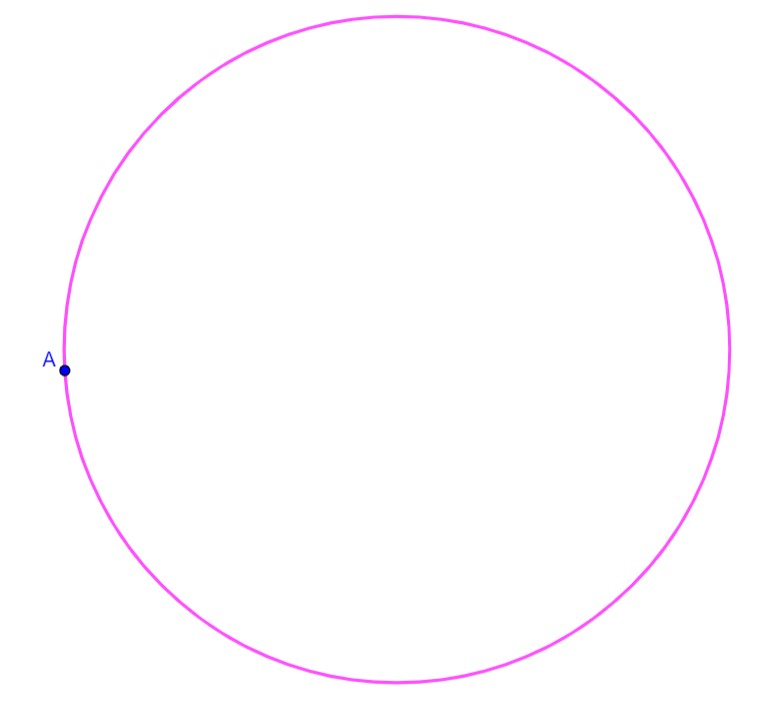
\includegraphics[scale=0.6]{circle_1.jpg}
	\end{figure}
\end{center}
If \(S\) is a circle, then \(S\) is a simple closed curve that exists in a 2-dimensional subspace of \(\R^3\).  Since a 2D subspace of \(\R^3\) is isomorphic to \(\R^2\), the Jordan curve theorem implies \(S\) divides this subspace into two regions, a region interior to \(S\) and a region exterior to \(S\).
\\[2\baselineskip]
2. Pick a direction, that is, a vector, \(v\), that lands you in the region interior to \(S\) and construct the ray with origin \(A\) eminating in the direction of \(v\).  For example,
\begin{center}
	\begin{figure}[h]
		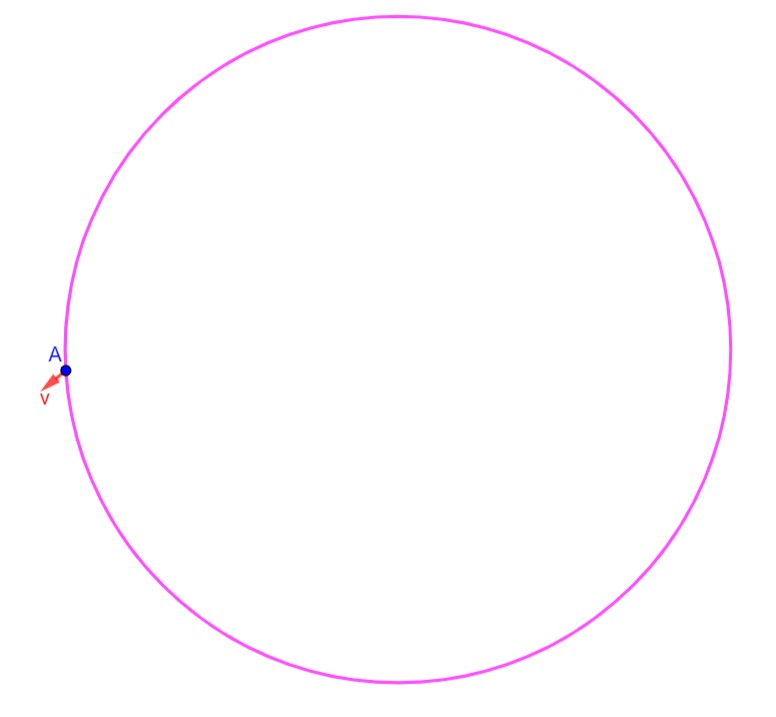
\includegraphics[scale=0.6]{circle_2.jpg}
	\end{figure}
\end{center}
is not a valid direction, whereas
\begin{center}
	\begin{figure}[h]
		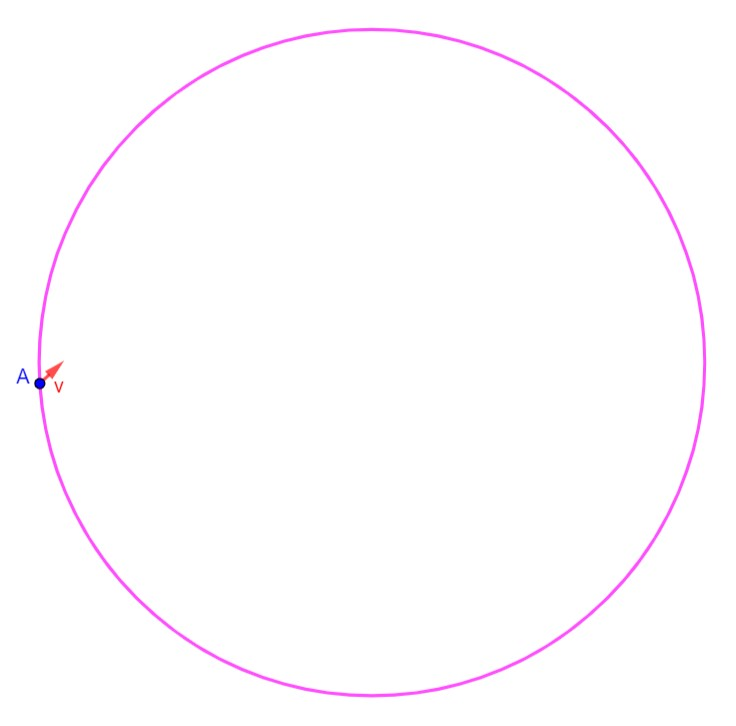
\includegraphics[scale=0.59]{circle_3.jpg}
	\end{figure}
\end{center}
is a valid direction.
\newpage
We then obtain the ray, \(R_1\), and the intersection point, \(B\).  
\begin{center}
	\begin{figure}[h]
		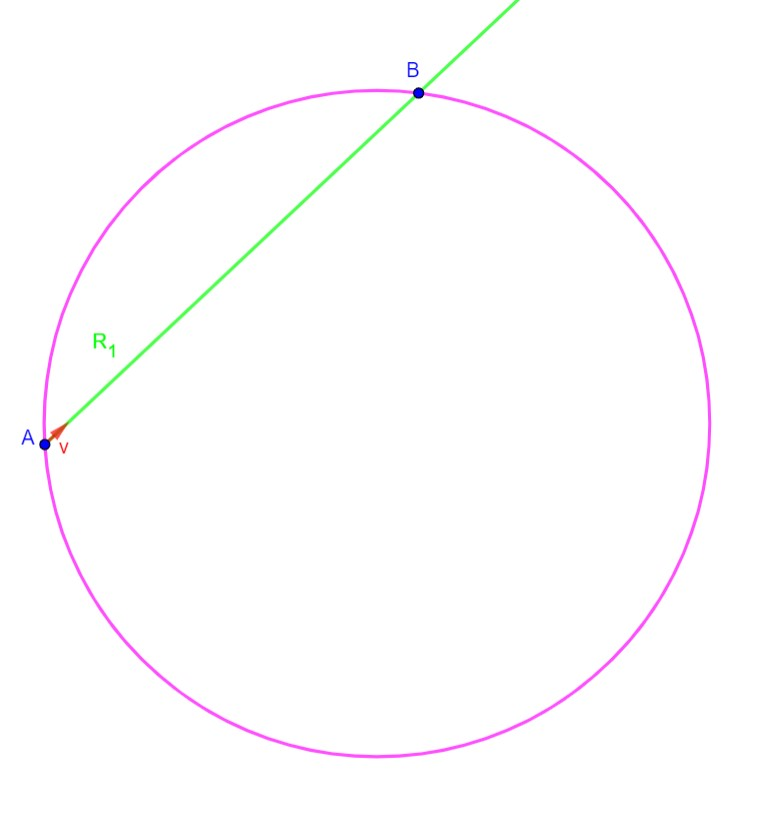
\includegraphics[scale=0.5]{circle_4.jpg}
	\end{figure}
\end{center}
3. At the point \(B\), construct the line, \(R_2\), passing through \(B\), perpendicular to \(R_1\). Label the point of intersection of \(R_2\) and \(S\) that is not equal to \(B\), \(C\).
\begin{center}
	\begin{figure}[h]
		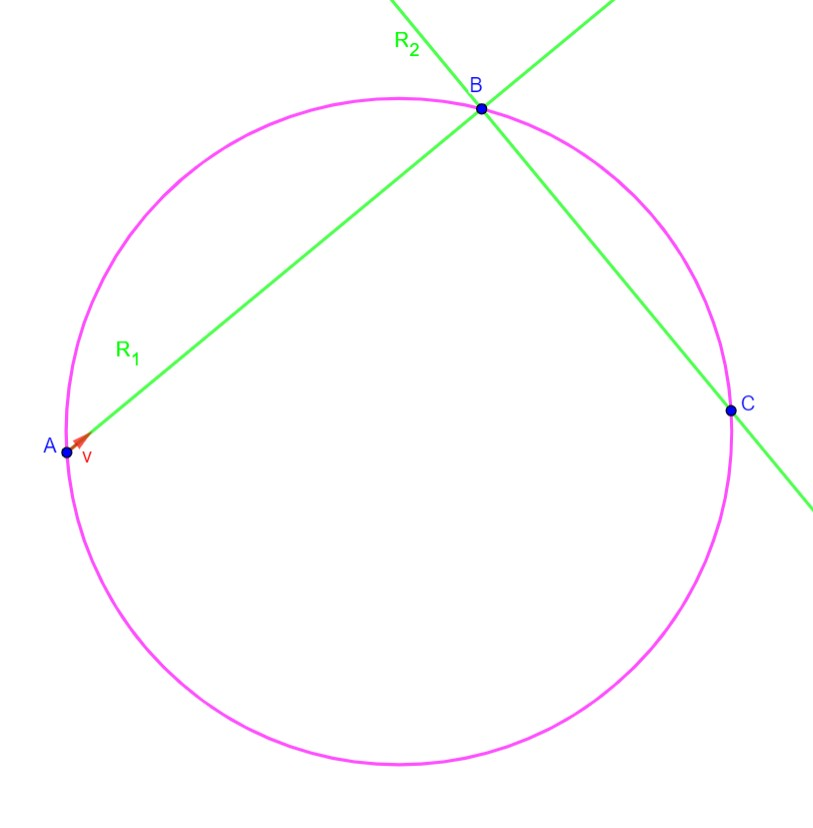
\includegraphics[scale=0.5]{circle_5.jpg}
	\end{figure}
\end{center}
In the event that there is not another point, \(C\), intersecting \(S\), different from \(B\), than \(R_2\) is tangent to \(S\) at \(B\).  In this case, \(AB\) gives a diameter of \(S\), and \(r=\frac{1}{2}length(AB)\) gives the radius of \(S\).
\begin{center}
	\begin{figure}[h]
		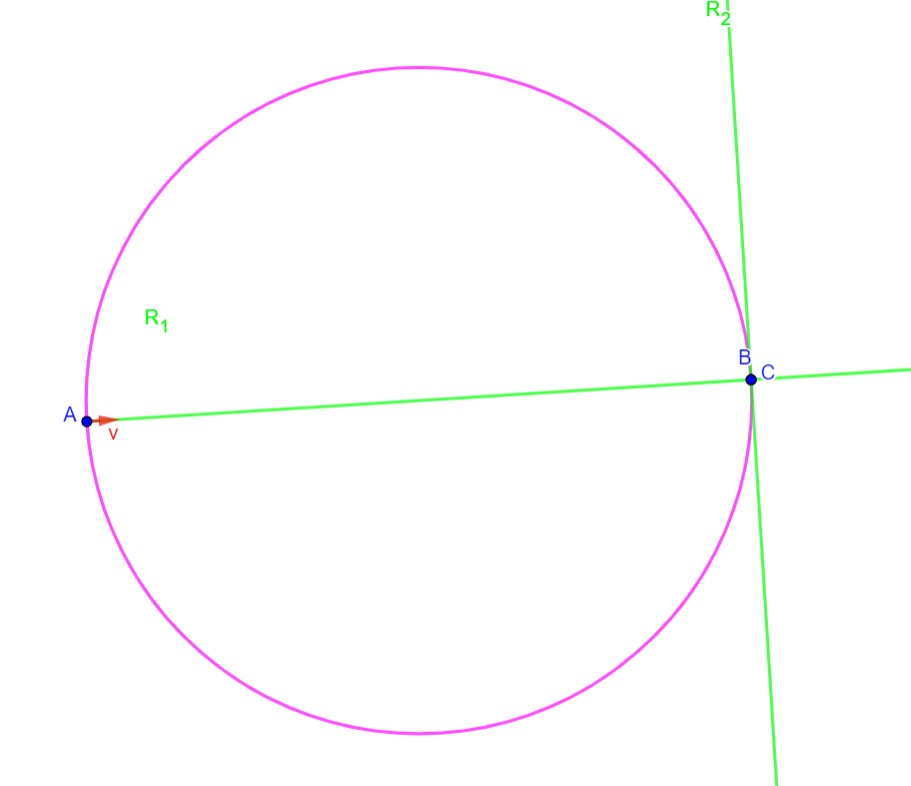
\includegraphics[scale=0.5]{circle_5_b.jpg}
	\end{figure}
\end{center}
Otherwise, construct the line segment \(AC\).  Since the inscribed angle, \(\angle ABC\), is \(90^{\circ}\) by construction, the central angle with inscribed points \(A\) and \(C\) must be \(180^{\circ}\).  Hence \(AC\) is a diameter of \(S\). 
\begin{center}
	\begin{figure}[h]
		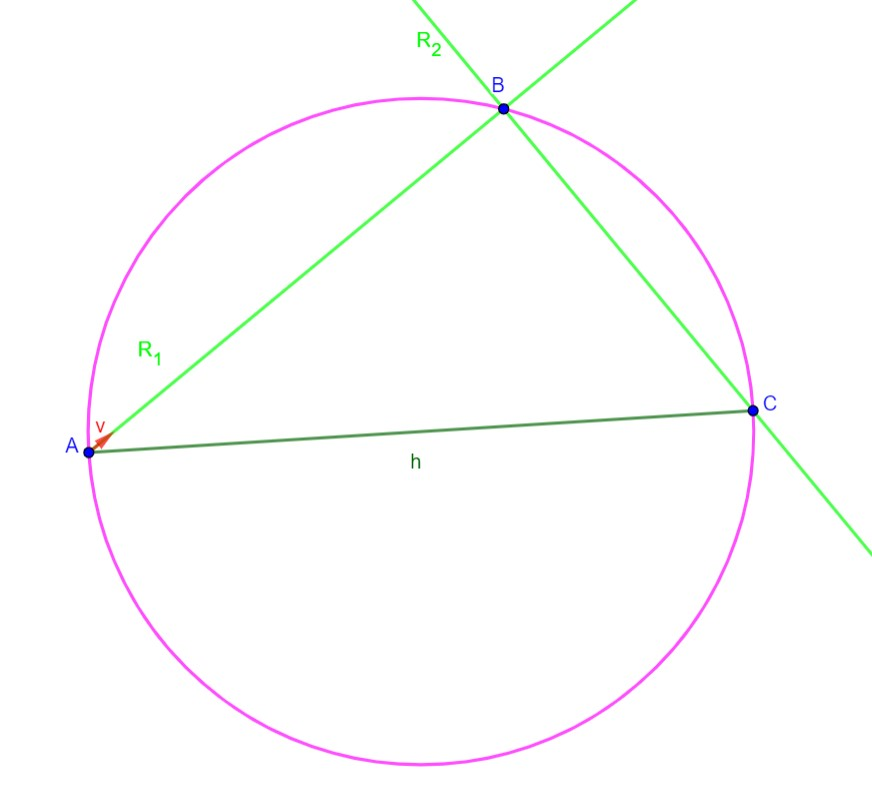
\includegraphics[scale=0.5]{circle_6.jpg}
	\end{figure}
\end{center}
We can then take \(r = \frac{1}{2}length(AC)\) as the radius of \(S\).
\newpage
Another way we could find the radius of our supposed circle, \(S\), is to pick a point, \(A\), on \(S\), construct the line tangent to \(S\) and \(A\) and then construct the line perpendicular to this tangent line at \(A\).  We can then label the second intersection of \(S\) with this perpendicular line as \(B\).  Since lines tangent to a circle are perpendicular to  radial lines at the point of tangency, \(AB\) is a diameter of \(S\) and we may take \(r=\frac{1}{2}length(AB)\) as the radius for \(S\).  We know such a point, \(B\), will exist since \(S\) is compact and the distance function is continuous.
\begin{center}
	\begin{figure}[h]
		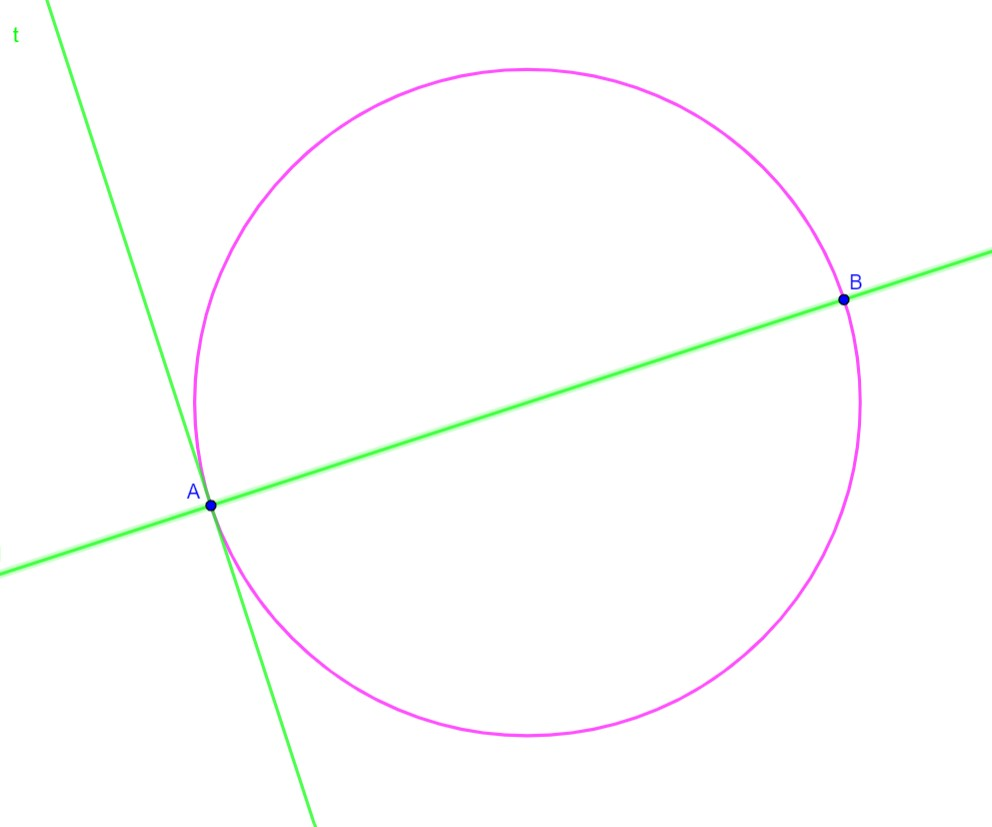
\includegraphics[scale=0.5]{circle_2_1.jpg}
	\end{figure}
\end{center}
Once we have our radius, \(r\), we then use inscribed, regular \(n\)-gons to get approximations of our circle. We can inscribe a regular \(n\)-gon in a circle, \(S\), of radius \(r\) as follows:
\\[1\baselineskip]
1. Pick a point on \(S\).  Using the fact that an interior angle of a regular \(n\)-gon has measure \(\alpha = ((\frac{n-2}{n})\cdot 180)^{\circ}\), from the diameter constructed in obtaining the radius of \(S\), rotate \((\frac{1}{2}(\frac{n-2}{n})\cdot 180)^{\circ}\) in either direction.
\\[1\baselineskip]
We aim to construct a side of our regular \(n\)-gon after performing this angle rotation.  Note, a regular \(n\)-gon can be divided up into \(n\) equal isosceles triangles with the equal side lengths equal to the radius of our circle, and angle between these sides equal to \(\frac{360}{n}^{\circ}\) 
\begin{center}
	\begin{figure}[h]
		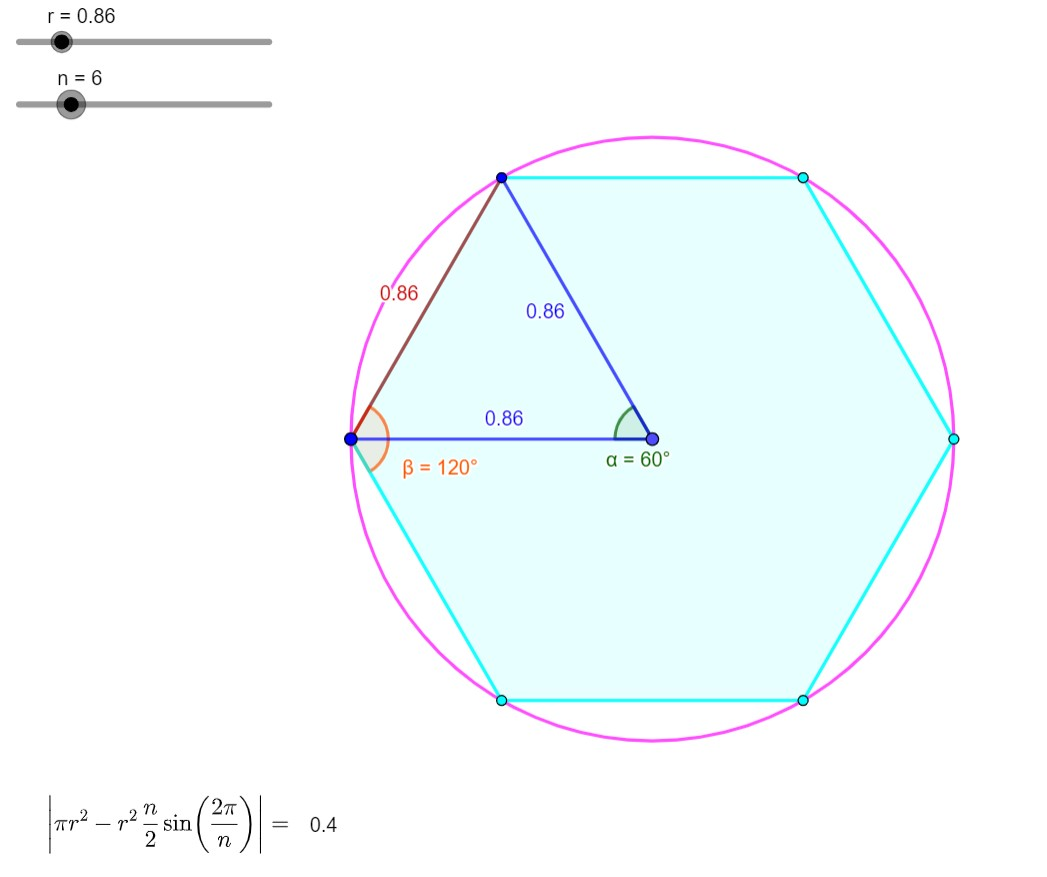
\includegraphics[scale=0.25]{circle_8.jpg}
	\end{figure}
\end{center}
In an isosceles triangle, we can find the length of the third side according to
\begin{center}
	\begin{figure}[h]
		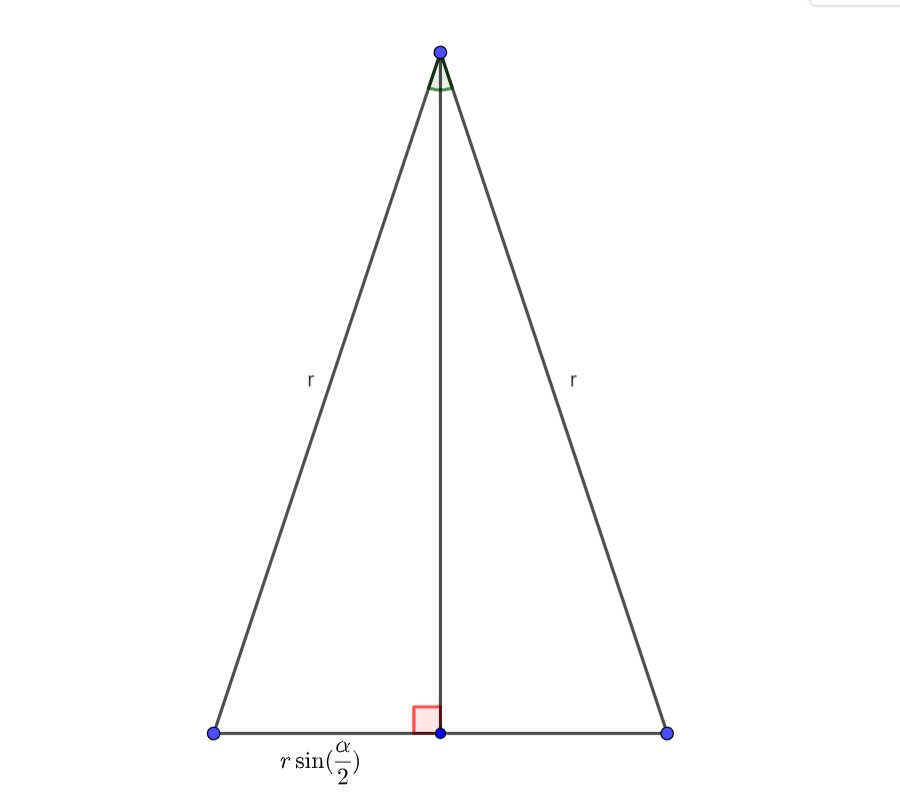
\includegraphics[scale=0.5]{isos.jpg}
	\end{figure}
\end{center}
So that the length of each side in our regular \(n\)-gon is \(2r\sin\left( \frac{\pi}{n} \right)\).
\\[1\baselineskip]
2. After rotating \((\frac{1}{2}(\frac{n-2}{n})\cdot 180)^{\circ}\) from the diameter of \(S\), construct a line segment of length \(2r\sin\left( \frac{\pi}{n} \right)\).  If \(S\) is a circle, this line segment should land back on \(S\).  If this line segment does not land back on \(S\), you can conclude \(S\) is not a circle.
\\[1\baselineskip]
3. If the line segment constructed lands you back on \(S\), rotate \(((\frac{n-2}{n})\cdot 180)^{\circ}\) so that the terminal ray lies in the region interior to \(S\).  Construct a line segment of length \(2r\sin\left( \frac{\pi}{n} \right)\).  If \(S\) is a circle, this line segment should land back on \(S\).  If this line segment does not land back on \(S\), you can conclude \(S\) is not a circle. 
\\[1\baselineskip]
4. Repeat step 3 a total of \(n-2\) more times.  If at any point the line segment construction does not land back on \(S\), or at any point the line segment constructed crosses \(S\) before fully constructed, you can conclude \(S\) is not a circle.  If after completing \(n\) total side constructions you do not return to your starting point, you can conclude \(S\) is not a circle.
\begin{center}
	\begin{figure}[h]
		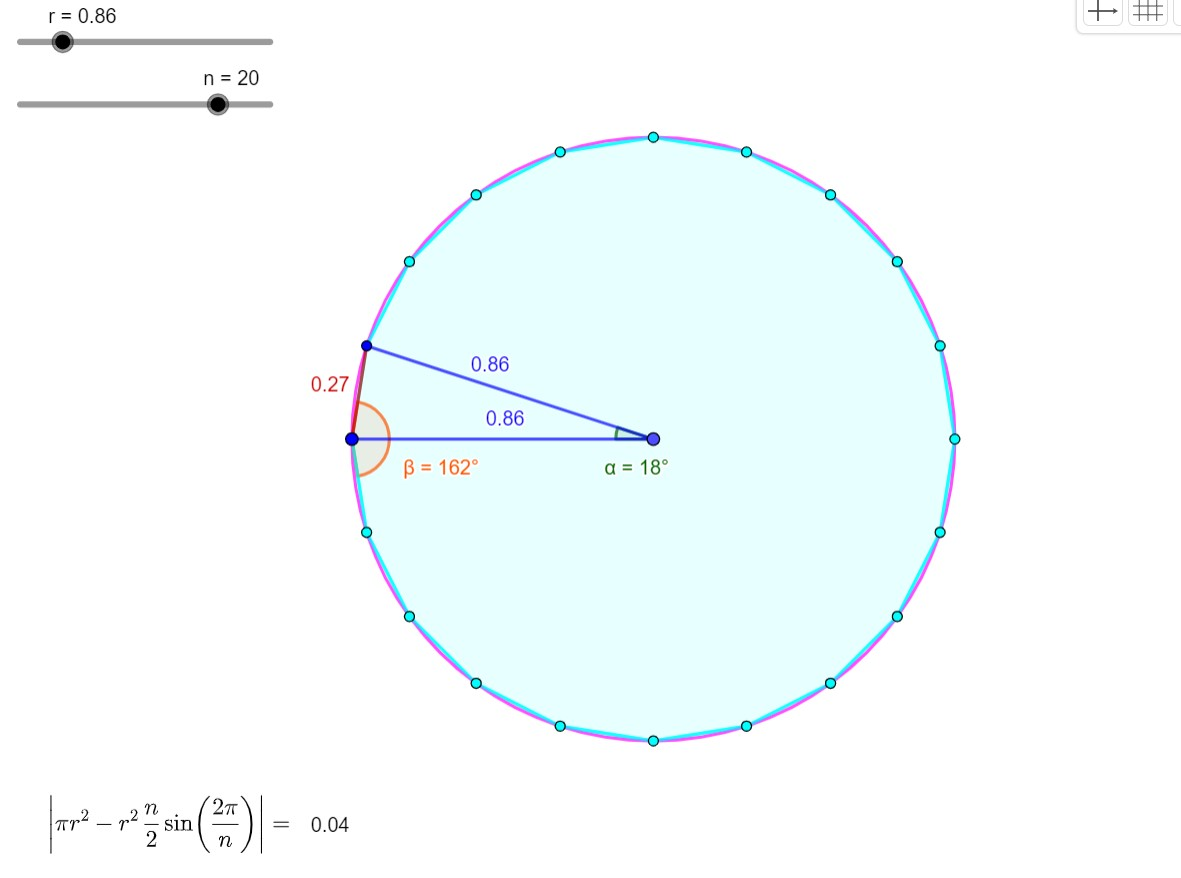
\includegraphics[scale=0.29]{circle_7.jpg}
	\end{figure}
\end{center}
\end{document}








